\chapter{Databases design}

%TODO INCLUDE PDF WHEN COMPILING
%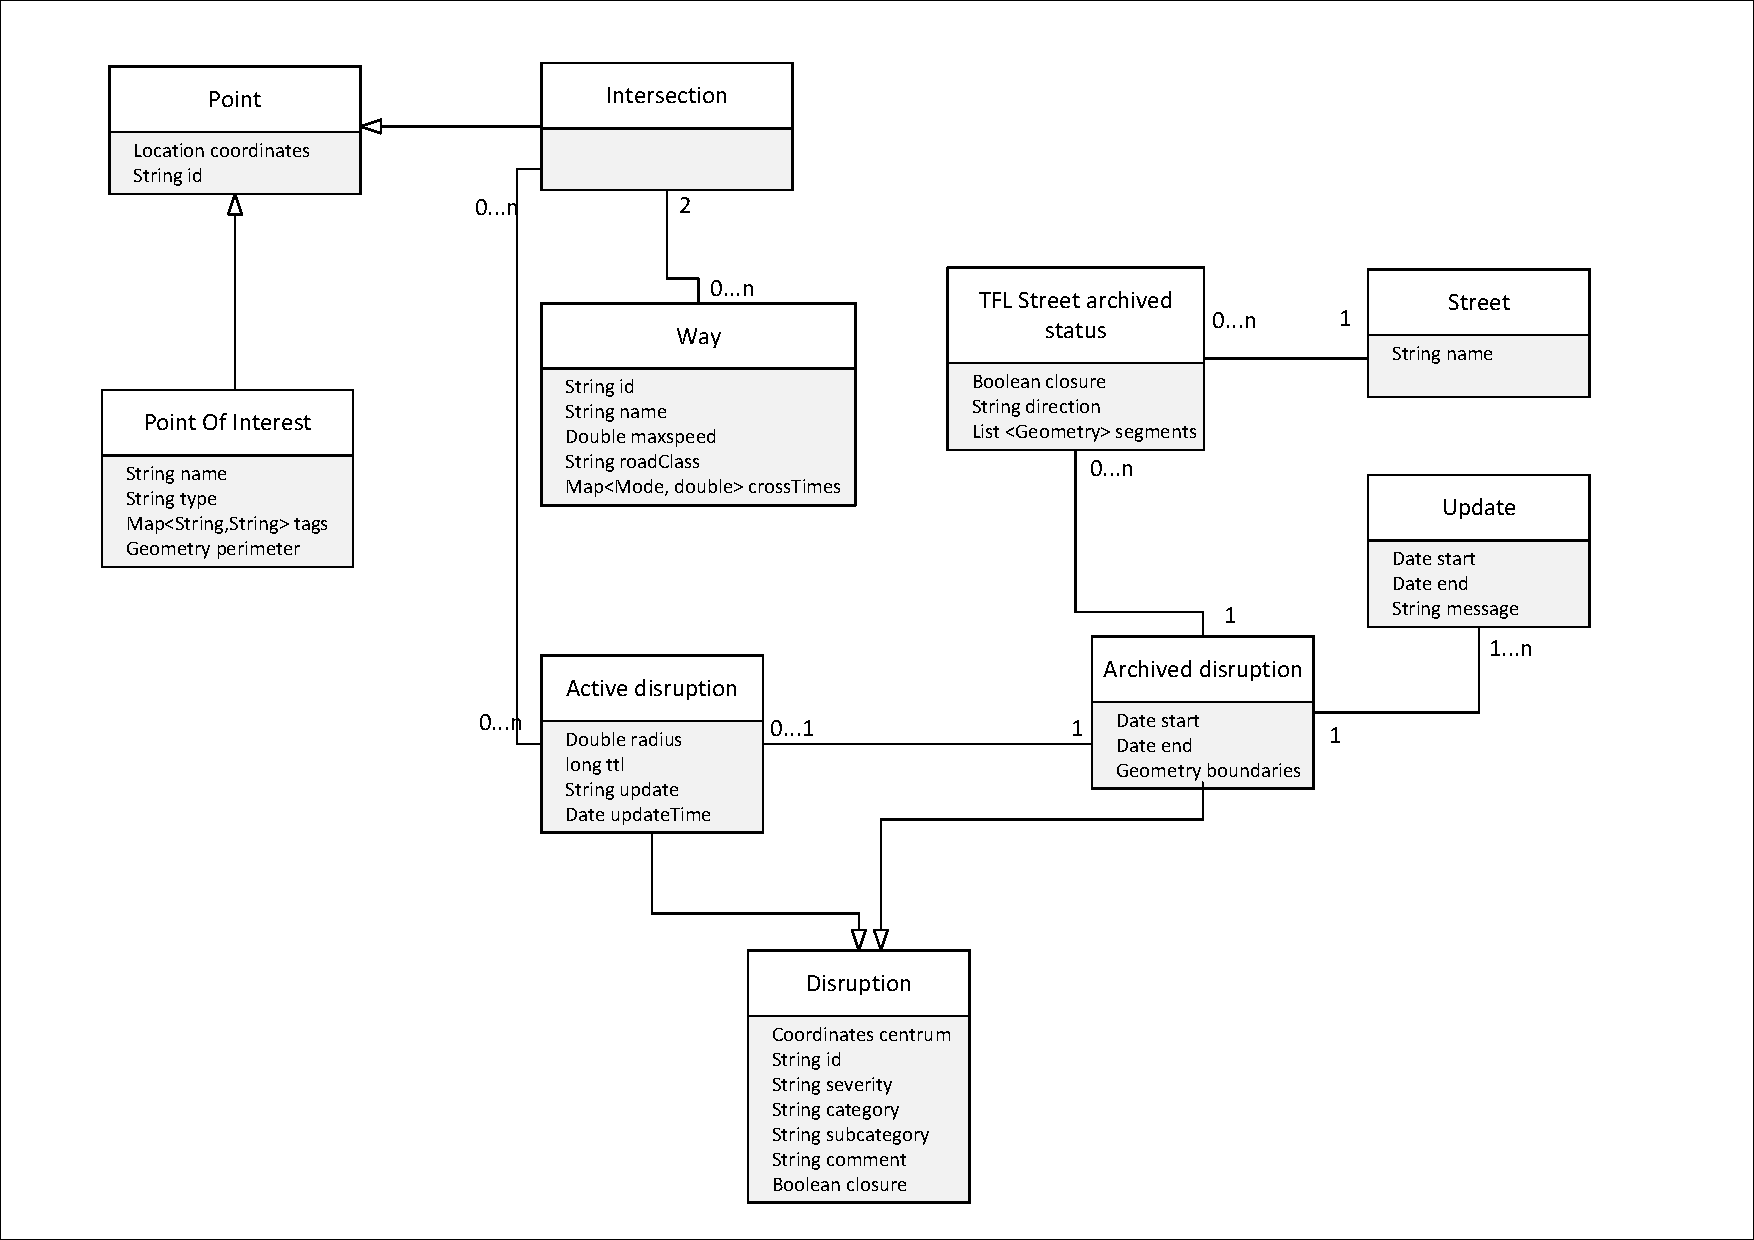
\includepdf[landscape=true,pagecommand=\thispagestyle{plain}]{assets/uml.pdf}

\chapter{Data model}

\paragraph{}
The data model section includes a description of the document collections, 
graph nodes and keys that are stored in the database. Two types of DBMSes have 
been selected for this purpose. 

\paragraph{Document DB}
MongoDB has been chosen as the database management system for the document 
database part, which stores information about the Point Of Interest and the 
concluded disruptions.

The decision to use a document database was based on its flexibility and 
ability to perform complex queries and works as a way to store an history of 
these informations.

\paragraph{Graph DB}
To manage the routing, where users can insert two points and the application will compute a travel route between them, a graph database managed using Neo4j has been selected to better support these features.

\section{Document database}

\paragraph{DBMS} Our choice for the \textit{database management system} to 
handle the document database was \textit{MongoDB}, since it is the most popular 
\textit{DBMS} of its kind and it also provides several functionalities useful 
for our use case, such as indexes and a powerful query engine.

\paragraph{Collections} In MongoDB we created the following collections:

\begin{itemize}
	\item POIs
	\item Disruptions
\end{itemize}

The POIs collection looks like this:
\begin{lstlisting}
{
	"_id":
	"name":
	"type":
	"coordinates": {
		"type": "Point",
		"coordinates": [0.0, 0.0] // lat 'n lon
	}
}
\end{lstlisting}

The disruption collection is organized in the following structure:
\begin{lstlisting}
{
	"idDisruption":
	"type":
	"startTime":
	"endTime":
	"coordinates": {
		"type": "Point",
		"coordinates": [0.0, 0.0] // lat 'n lon
	},
	"boundaries": {
		"type": "Polygon",
		"coordinates": [
		[
		[100.0, 0.0],
		[101.0, 0.0],
		[101.0, 1.0],
		[100.0, 1.0],
		[100.0, 0.0]
		]
		]
	}
	
	,
	
	"category":
	"subcategory":
	"severity":
	"updates": [{
		"startTime":
		"endTime":
		"message":
	},
	
	]
	"streets": [{
		"name":
		"closure":
	},
	{
		"name":
		"closure":
	},
	..
	]
	"closure":
	
}
\end{lstlisting}
This representation might allow in the future to store additional optional values for certain kinds of POIs if the need arises, without any compatibility issue for the existing code; for example one might want to store a restaurant’s opening hours or the accessibility level for wheelchair users in a certain building.

\section{Graph database}

\paragraph{DBMS} Our choice for the \textit{database management system} to 
handle the graph database was \textit{Neo4j}, since it can easly handle a huge amount of nodes.


\paragraph{Data} The graph DB is mainly used to store the road network of London and the current active disruption, this is needed so that the routing algorithm can avoid adding to the frontier nodes in an area affected by a closure or increase the weight of nodes in areas affected by critical disruptions.

\paragraph{Schema}For the map side of things we store one class of node and one class of relationship:

\begin{itemize}
	\item \textbf{Intersection }(due to a mistake it is actually called Point in the database) represents the connection between one or more ways, it is a \textit{vertex} of the graph
	\item \textbf{Connects} represents the connection between two Insersection. It stores informations like its name and the cost of traversing it and eventual access restrictions, like one way streets or motor-only roads
	
\end{itemize}

For the disruption handling we have the following nodes and relationships:

\begin{itemize}
	\item \textbf{Disruption} a node in the graph containing all the informations about an active disruption
	\item \textbf{isDisrupted} is a relation between a Point and a Disruption, telling that the road is being affected by a disruption

\end{itemize}
	
\begin{figure}[H]
	\centering
	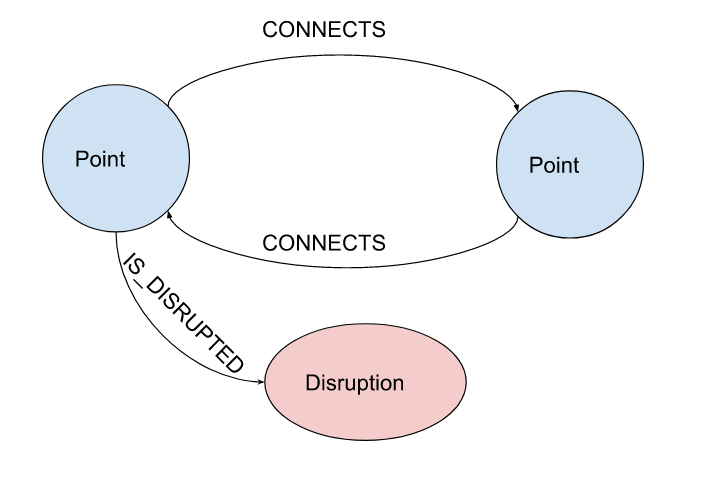
\includegraphics[width=0.7\linewidth]{assets/schemaneo4j}
	\caption{A possible portion of graph}
	\label{fig:schemaneo4j}
\end{figure}

